%% allgemeine Textformatierung

\documentclass[
	oneside,			%				einseitig
	a4paper,			%				DIN A4-Format
	12pt				%				Schriftgr��e
%]{report}
]{scrreprt}
%]{book}

% F�r die Verzeichnisse f�r Abk�rzungen, Fremdw�rter, Symbole
%\usepackage[]{artlos,artlob,artlow}

%% deutsche Sprachanpassungen (Silbentrennung, Umlaute usw.)
\usepackage{ngerman}

%% keine Ahnung, is aber immer drin :-)
\usepackage[T1]{fontenc}
\usepackage[latin1]{inputenc}

%% nicht bitmap, sondern postscript (type 1, vector)
\usepackage[]{pslatex}

%% Package zum einf�rben von Text und anderen Objekte
%\usepackage{color}

%% Package zum einbinden von Grafiken
\usepackage[]{graphicx}

%% Package f�r Index (Register)
\usepackage{makeidx}
\makeindex
\renewcommand{\indexname}{Stichwortverzeichnis}

%% Package f�r Kopfzeilen
\usepackage{fancyhdr}
% Kopfzeilenformat festlegen
\rhead{}
\headheight = 14.5pt

%% Package zum einbetten von Verweisen in die Ausgabe (DVI, PDF)
\usepackage[
	bookmarksopen=true,			% �ffnet alle Lesezeichen (nur in PDF)
	plainpages=false				% erm�glicht mehrere Seitenzahlformate
]{hyperref}

%% Package f�r Abk�rzungsverzeichnis (Glossar)
\usepackage{nomencl}
	\let\abbrev\nomenclature
	\renewcommand{\nomname}{Abk�rzungsverzeichnis}
	\setlength{\nomlabelwidth}{.25\hsize}
%	\renewcommand{\nomlabel}[1]{#1 \dotfill}
	\setlength{\nomitemsep}{-\parsep}
% Paketabhaengig heissen die Befehle makenomenclature / printnomenclature
%                 oder makeglossary / printglossary !!!!
	% \makenomenclature
	\makeglossary
%	\let\listofabbreviations\printnomenclature  % Paketabhaengig !!!!
	\let\listofabbreviations\printglossary

%% Hervorhebung f�r das Abk�rzungsverzeichnis
\usepackage[normalem]{ulem}
	\newcommand{\markup}[1]{\underline{#1}}

% Seitenformat festlegen
\textwidth14.5cm
\textheight24.5cm
\topmargin-15mm

% 1.5 zeilig
\linespread{1.25}\selectfont

%% Package zum formatieren von Tabellen
\usepackage{array}

% kein Einr�cken am Absatzanfang
\parindent 0pt 

% variabler Abstand zwischen W�rtern, um Blocksatz zu wahren und weniger zu trennen
\sloppy
	

% eigene

\usepackage{enumitem}% http://ctan.org/pkg/enumitem
\usepackage{pdflscape}
\usepackage{hyperref}
\usepackage{url}

\include{csquote.sty}
\usepackage{csquotes}

\usepackage{listings}
\newcommand{\code}[1]{\texttt{#1}}

\usepackage{xcolor}


%\usepackage{biblatex}
%\addbibresource{Kapitel/Literatur.bib}

%

\begin{document}

\begin{titlepage}
\vspace{0cm}
      \begin{figure}[h]
        \begin{flushright}
          
\includegraphics[width=11em]{pics/logo}
        \end{flushright}
      \end{figure}
    \vspace{1cm}
    {\centering \textsf{\Large Fakult�t f�r Ingenieurwissenschaften}\par}
    \vspace{0.6cm}
%   {\centering \textbf{\Large \textsf{Diplomarbeit}}\Large \par}
%    {\centering \textbf{\Large \textsf{Bachelor-Thesis}}\Large \par}
   {\centering \textbf{\Large \textsf{Expos� zur Master-Thesis}}\Large \par}
    \vspace{0.2cm}
            {\centering {\Large \textsf{Automating ROP and JOP Chain Generation\\
            aka ROP Compiler}}\par}
    \vspace{2cm}

            \begin{tabular}{p{5cm}l}
                eingereicht von:    & David Schunke\\
                                    & Studiengang IT-Sicherheit und Forensik\\
                Matrikelnummer:     & 417785\\
            \end{tabular}

    \vspace{1.25cm}
\end{titlepage}

\pagestyle{fancy}

%%%%%%%%%% PRE %%%%%%%%%%%

\tableofcontents{}
%\addtocontents{toc}{\protect\addcontentsline{toc}{chapter}{Inhaltsverzeichnis}}

%%%%%%%% MAIN %%%%%%%%%%%%%%%%%%%
 
\chapter{Problemstellung und Motivation}

\emph{Return-oriented-programming (ROP)} und \emph{Jump-oriented-programming (JOP)} sind Angriffstechniken, welche genutzt werden, um Schadcode trotz vorhandener Sicherheitsmechanismen ausf�hren zu k�nnen. Dies erfordert im Zielprogramm eine Verwundbarkeit im Bereich Memory Corruption (z.B. Buffer Overflow, Use-After-Free (UAF), o.�.). Hierzu werden die im Zielprogramm vorhandenen Programmanweisungen (Assembler-Instruktionen / Opcode / Machine Code TODO), welche sich bereits im Programmspeicher befinden, genutzt, um sogenannte \emph{ROP Gadgets} [TODO Footnote] zu bilden.\\
Ein Gadget ist eine kleine Code Sequenz, welche eine bestimmte Aufgabe durchf�hrt, z.B. das Kopieren eines Speicherregisters in ein Anderes oder die Addition zweier Register. ROP oder JOP Gadgets enden typischerweise mit einer \emph{return}, \emph{jump} oder \emph{call} Anweisung, welche die Ausf�hrung zu einer vorherig gespeicherten Stelle zur�ckbringen soll. Durch Manipulation dieser Return-Addresse erlaubt es dem Angreifer Gadgets zu verketten, um eigene Operationen durchzuf�hren und ein gew�nschtes Ergebnis zu erzielen. Da lediglich Maschineninstruktionen genutzt werden, welche sich bereits im Speicher des Programms befinden, k�nnen viele Sicherheitsmechanismen, wie z.B. NX, W\textasciicircum X oder DEP [TODO Footnote], umgangen werden.\\

Die Entwicklung eines ROP-basierten Exploit erfordert es bisher manuell ROP Gadgets zu verketten - d.h. Chains zu bilden - sowie den passenden Program Input zu finden, um �ber eine Memory Corruption die ROP Chain zu starten. Diese Prozesse durchzuf�hren ist nicht nur aus Angreifersicht von Interesse, sondern auch aus Sicht von Sicherheitsforschern (White Heads / Blue / Red Teams) wichtig, um m�gliche Exploits finden und anschlie�end beheben bzw. melden zu k�nnen.\\

Die manuelle Suche einer ROP Chain ist zeitintensiv und erfordert tiefgreifende Kenntnisse der zugrundeliegenden Architektur, des Zielprogramms sowie der Funktionsweise von Maschinenprozessen und Speicherverwaltung. An die durchf�hrende Person werden somit hohe Anforderungen gestellt, welche das eigentliche Auffinden von Schwachstellen erschwert.\\

Durch die Erstellung eines \emph{ROP Compilers} k�nnten diese Prozesse schrittweise automatisiert werden. Dies w�rde den zeitlichen Aufwand verringern sowie die M�glichkeit des Nachweises einer Schwachstelle mittels eines Exploits bzw. PoC an eine breitere Masse von Personen geben, um so Schwachstellen schneller finden, beheben als auch im Bereich der Strafverfolgung sowie Nachrichtendienste nutzen zu k�nnen.
\chapter{Ziele und Grenzen}

\section{Zielsetzung}

Im Rahmen dieser Arbeit soll ein ROP Compiler entwickelt werden, welcher als Eingaben auf zur Verf�gung stehender Gadgets sowie vordefiniertem Code basierend eine Verkettung der Gadgets automatisiert durchf�hren soll. Die zur Verkettung ben�tigte Semantik sowie die zur Eingabe ben�tigten Formatregeln sollen ebenfalls innerhalb dieser Arbeit definiert und implementiert werden.\\

Ziel ist die Erstellung eines Proof-of-concept (PoC), welcher auf Basis einer zuvor ausgew�hlten spezifischen Prozessorarchitektur (X64, ARM32 oder ARM64) die grunds�tzliche Umsetzbarkeit demonstrieren und Ausgangspunkt f�r weitere Arbeiten bilden soll.\\

Au�erdem soll der Grad der Berechenbarkeit er�rtert und gezeigt werden, dass - abh�ngig vom zugrundeliegenden Zielprogramms, welches exploited werden soll - eine Touring-Vollst�ndigkeit nicht grunds�tzlich vorliegt.\\

Anhand verschiedener konstruierter sowie realer Beispiele soll der PoC evaluiert und die Umsetzbarkeit eines ROP Compilers nachgewiesen werden.\\

Zum Schluss werden die Ergebnisse mit anderen ROP Compilern verglichen und die Unterschiede in Performance sowie Qualit�t evaluiert.

\section{Abgrenzung}

In dieser Arbeit wird die Findung von ROP Gadgets nicht betrachtet, sondern durch bereits bestehende Projekte, welche innerhalb der Arbeit vorgestellt und referenziert werden sollen, zur weiteren Verarbeitung vorgegeben.\\

Des Weiteren wird sich in dieser Arbeit ausschlie�lich auf eine Prozessorarchitektur spezifiziert, da diese sich tiefgehend in den zugrundeliegenden Techniken unterscheiden. Ein universeller ROP Compiler kann daher in dieser Arbeit nicht entwickelt werden, bildet aber M�glichkeit f�r nachfolgende Projekte.
\chapter{Stand der Forschung}

ROP und JOP sind Techniken, welche bereits seit Ende der 90er Jahre genutzt werden. Einer der wohl bekanntesten Exploits auf ROP Basis ist der return-into-libc Overflow Exploit \cite{ret2libc}.\\

F�r das Auffinden von Gadgets gibt es ebenfalls bekannte Projekte, welche in der Lage sind teilweise f�r verschiedene Prozessorarchitekturen Gadgets aus einer gegebenen Binary zu finden und anzeigen zu lassen. Ein Beispiel f�r solch ein Projekt w�ren ROPgadget \cite{JonathanSalwan/ROPgadget} oder Ropper \cite{sashs/Ropper}.\\

\emph{Q} \cite{schwartz2011q} war eine Forschungsarbeit der Carnegie Mellon University in Pittsburgh. In diesem Projekt wurden \enquote{semantic program verification techniques} genutzt, um einen gegebenen Exploit, welcher durch Sicherheitsmechanismen wie W$\oplus$X verhindert wird, in eine ROP Chain abzubilden, um den \enquote{Exploit zu h�rten} (exploit hardening). Ans�tze der Semantik zur Verkettung k�nnen eventuell f�r diese Arbeit interessant werden.\\

angrop \cite{angr/angrop} ist ein Tool zum Auffinden von ROP Gadgets. Au�erdem soll es ROP Chains automatisch verketten k�nnen. Es nutzt das Binary Analysis Framework angr \cite{angr}, welches von verschiedenen Forschern vom Computer Security Lab der UC Santa Barbara sowie dem SEFCOM der Arizona State University entwickelt wird. Gef�rdert wurde das Projekt von der U.S. Regierung. Die Ergebnisse wurden unter open source gestellt \cite{shoshitaishvili2016state}. angrop verfolgt den gleichen Ansatz von \emph{Q} mit einigen kleineren Abweichungen und Erweiterungen.\\

\emph{GENROP} \cite{branting2022rop} war Thema einer Masterthesis an der Link�ping University in Schweden. Das Thema von GENROP war sehr �hnlich zu dieser Arbeit und verfolgte den Ansatz Genetic Programming zum Verketten der ROP Gadgets zu nutzen. Das Ergebnis von GENROP war allerdings, dass die eigentlichen Kernkonzepte von Genetic Programming am Ende nicht mehr richtig genutzt werden konnten, um das Problem zu l�sen, da der Algorithmus zu sehr gelenkt werden musste. Genauere Einarbeitung und Analyse, welche Probleme bei GENROP auftraten, m�ssen noch erfolgen. Die Implementation des Projekts ist allerdings nicht �ffentlich verf�gbar.\\

Pure-Call Oriented Programming (PCOP) \cite{sadeghi2018pure} fokussiert sich auf Jump-oriented Programming (JOP) und somit Gadgets, welche in einer \code{call} Anweisung enden. Call Anweisungen werden vom Prozessor umgesetzt, indem die Speicheradresse der auf den Call direkt folgenden Anweisung auf den Memory Stack gelegt und eine \code{jmp} Anweisung zu der gew�nschten Speicheradresse ausgef�hrt wird. Dadurch, dass der Stack ver�ndert wird, ergeben sich Seiteneffekte, welche die Gadget Chain st�ren k�nnen. PCOP soll einige dieser Seiteneffekte beheben k�nnen. Au�erdem soll PCOP Touring-Vollst�ndigkeit besitzen, was bedeuten w�rde, dass beliebiger Code hierdurch emuliert werden k�nnte. Die genauen Ans�tze in diesem Artikel m�ssen im weiteren Verlauf noch herausgearbeitet werden.\\

Am Massachusetts Institue of Technology (MIT) wurde ein ROP Compiler \cite{stewart2015rop} erarbeitet, welcher die verf�gbaren Gadgets zuerst klassifiziert (basierend auf Logik aus \emph{Q} \cite{schwartz2011q}) und anschlie�end �ber die klassifizierten Gadgets iteriert. Au�erdem soll der vom MIT sogenannte \emph{Gadget Scheduler} auch bestimmte Speicherregister beobachten, sodass keine gegenseitigen �berschreibungen stattfinden sollen. Das Projekt soll auf konstruierten Beispielen sowie auf \code{rsync} als real-world Binary erfolgreich als PoC umgesetzt werden. Leider ist lediglich der Artikel und nicht die Codebasis �ffentlich verf�gbar.\\

Multi-Architecture JOP and ROP Chain Assembler (MAJORCA) \cite{nurmukhametov2021majorca} war ein Projekt des Moscow Institue of Physiscs and Technology, welches \enquote{spezielle Graphe zur Suche nach \code{mov} Ketten} zur Bildung der Gadget Chains genutzt hat. W�hrend sich dieses Projekt allerdings auf die x86 Architektur fokussiert, k�nnen Ideen und Ans�tze hieraus eventuell auch f�r diese Masterthesis interessant sein.\\

Im Rahmen der weiteren Vor- und Recherchearbeiten sollen die einzelnen Techniken der vorgestellten sowie weiterer Arbeiten genauer herausgearbeitet, verglichen sowie f�r die Bildung der Semantik in dieser Arbeit herangezogen werden.
\chapter{Vorarbeiten}

Diese Abschlussarbeit wird in Kooperation mit der Zentralen Stelle f�r Informationstechnik im Sicherheitsbereich (ZITiS) erstellt. Hierzu wurde bereits Kontakt mit der ZITiS aufgenommen sowie alle ben�tigten vertraglichen Grunds�tze gekl�rt. Der offizielle Vertragsbeginn mit der ZITiS wurde auf den 01.03.2023 festgelegt.\\

Zur Bearbeitung wurde bereits durch die ZITiS ein Betreuer festgelegt, mit welchem bereits ein erster Austausch stattgefunden hat. Des Weiteren soll durch die ZITiS ab offiziellem Vertragsbeginn Hardware sowie Zugang zu gewissen Informationen und Infrastruktur bereitgestellt werden.\\

Eine Einarbeitung in das Thema, die technischen Grundlagen sowie etwaige Suche von Quellen und verwandten Projekten, fand und findet bereits statt.
\chapter{Vorgehensweisen und Methoden}


\begin{landscape}

\chapter{Zeit und Arbeitsplan}

\begin{figure}
	\centering
	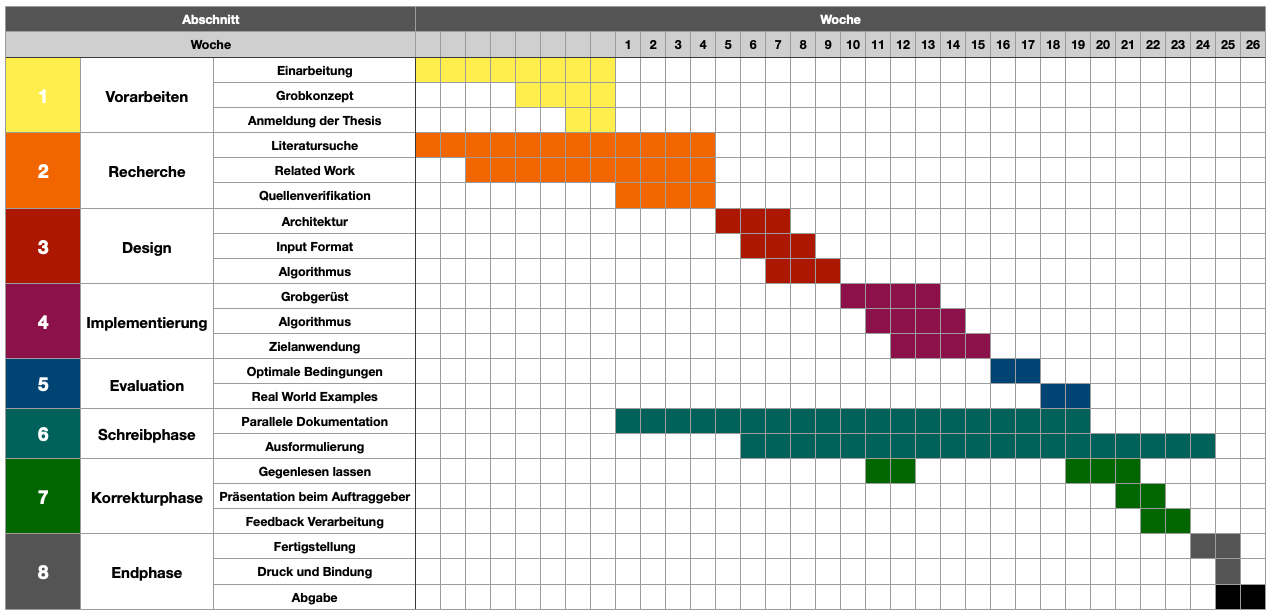
\includegraphics[trim=0 0 0 0, scale=0.3]{pics/Zeitplan}
\end{figure}

\end{landscape}

%%%%%%%%%%%%%%%%%%% POST %%%%%%%%%%%%%%%%%%%%%%

% Beginn Anhang
\appendix

\cleardoublepage
%\mycleardoublepage
\phantomsection
\addtocontents{toc}{\protect\vspace*{\baselineskip}}

\bibliographystyle{alphadin}
%\bibliographystyle{plain}
\addcontentsline{toc}{chapter}{Literatur}
\bibliography{Kapitel/Literatur}


%\listoffigures{}
%\addtocontents{lof}{\protect\addcontentsline{toc}{chapter}{Abbildungsverzeichnis}}

%\listoftables{}
%\addtocontents{lot}{\protect\addcontentsline{toc}{chapter}{Tabellenverzeichnis}}

%\pagestyle{myheadings}\markboth{}{}
%\phantomsection\listofsymbols
%\addtocontents{los}{\protect\addcontentsline{toc}{chapter}{\listofsymbolsname}}
%\phantomsection\listofakues
%\addtocontents{lob}{\protect\addcontentsline{toc}{chapter}{\listofakuesname}}
%\phantomsection\listoffremds
%\addtocontents{low}{\protect\addcontentsline{toc}{chapter}{\listoffremdsname}}

%%Abk�rzungsverzeichnis
%
% sortiert Abk�rzungen alphabetisch
% entfernt doppelte Eintr�ge
%
	\abbrev{ERM}{\markup{E}mpirical \markup{R}isc \markup{M}inimisation}
	\abbrev{XML}{E\markup{x}tensible \markup{M}arkup \markup{L}anguage}
	\abbrev{ABK}{\markup{Abk}�rzung} % der befehl \markup kann in der Config belibig angepasst werden in diesem Bsp unterstreicht er
	\nomenclature{ABK}{\markup{Abk}�rzung} %macht das Gleiche, \nomenclature ist der Orginalbefehl der in der Config auf \abbrev ge�ndert wurde

%\chapter{Appendix}

\index{foobar}

foobar

\end{document}
